\documentclass{report}

\usepackage{skesrsstyles}  % use styles from SKE SRS

% Add third-party packages
\usepackage{fontspec}
\setmainfont{Times New Roman}
\newfontfamily\thaifont{TH Sarabun New}[Scale=MatchLowercase]
\usepackage{ucharclasses}
\setTransitionsFor{Thai}{\thaifont}{\normalfont}
\usepackage[hidelinks]{hyperref}  % Allows hyperlink text in built document
\usepackage{url}  % Allows url line breaks
\usepackage{microtype}  % For hyphen-letterspacing configuration
\usepackage{amsmath}  % \text{} in math mode, displayed equations
\usepackage{cleveref}  % Smarter referencing (must load after amsmath)
\usepackage{graphicx}  % Allows insertions of graphics
\usepackage{tabularx}  % Better tabular environment, with dynamic column size support
\usepackage{indentfirst}  % Indent first paragraph after headers
\usepackage{enumitem}  % Better control of itemize, enumerate
\usepackage{pdflscape}  % Landscape pages for wide figures
\usepackage{multirow}   % Multi-row cells in tables
\usepackage{pifont}   % Dingbat symbols for comparison tables
\newcommand{\cmark}{\ding{51}}  % ✓
\newcommand{\xmark}{\ding{55}}  % ✗

\graphicspath{{./assets/}}

% add macro to substitute for empty vars
\def \usevar#1{\ifx\empty#1 \empty\else #1\fi}


%% -----------------------------------
% Edit the variables for the paper here!
\def \srsTitle{KUru: AI-Powered University Program Advisor for KU Program Selection using RAG, Knowledge Graph, and Hybrid Recommendation}
\def \srsTitleDisplay{KUru: AI-Powered University Program Advisor\\for KU Program Selection using RAG,\\Knowledge Graph, and Hybrid Recommendation}
\def \srsAuthorOne{Thanawat Tantijaroensin 6610545294}
\def \srsAuthorTwo{Phantawat Luengsiriwattana 6610545871}
\def \srsAuthorThree{}
\def \srsAcademicYear{2568}

\def \srsAdvisorName{Jitti Niramitranon}
\def \srsCoAdvisorName{}
\def \srsHoDName{Head of Department's Name}
%% -----------------------------------

\begin{document}

    \addtocontents{toc}{\moderate\noindent\textbf{Content}\hfill\textbf{Page}\par\addvspace{.2in}\normalsize}
    \addtocontents{lot}{~\hfill\textbf{Page}\par\addvspace{.2in}\normalsize}
    \addtocontents{lof}{~\hfill\textbf{Page}\par\addvspace{.2in}\normalsize}

    \newgeometry{hmargin={1in, 1in}, vmargin={1in, 1in}}
\thispagestyle{empty}
\begin{center}

    \includegraphics[width=1.7in]{assets/ku/symbol.png}\vspace{.45in}

    {\huge\textbf{SOFTWARE ENGINEERING PROJECT}}\vspace{.6in}

    {\huge\textbf{\usevar{\srsTitleDisplay} (Proposal)}}\vspace{.65in}

    {\huge\textbf{BY}}\vspace{.3in}

    {\huge\textbf{%
        \usevar{\srsAuthorOne} \\
        \usevar{\srsAuthorTwo}%
        \ifx\srsAuthorThree\empty\else \\ \usevar{\srsAuthorThree}\fi \\
    }}\vspace{.6in}

    {\Large\textbf{%
        DEPARTMENT OF COMPUTER ENGINEERING\\
        FACULTY OF ENGINEERING\\
        KASETSART UNIVERSITY\\
    }}\vspace{.3in}

    {\LARGE\textbf{Academic Year \usevar{\srsAcademicYear}}}

\end{center}
\restoregeometry
    \include{partials/innercover}

    \pagenumbering{roman}
    \setlength{\parindent}{40pt}

    %% PROPOSAL: Abstract and Acknowledgement hidden
    %% \chapter*{Abstract}
\label{chap:abstract}
\addcontentsline{toc}{chapter}{\nameref{chap:abstract}}

KUru is an AI-powered academic pathway navigation system for Kasetsart University (KU). The system addresses a clearly defined problem: students who are interested in exploring career paths or programs at KU lack personalized, structured guidance when selecting programs for TCAS applications.

The MVP employs a Retrieval-Augmented Generation (RAG) pipeline grounded in official KU curriculum, TCAS, and fee-related documents to enable semantic question-answering over program content in both Thai and English. An interest discovery interface grounded in Holland's RIASEC vocational model builds an initial student interest profile, which is used for simplified curriculum-side program recommendation through semantic matching. The target-system vision extends this MVP with a Neo4j knowledge graph, O*NET career matching, behavioural personalisation, portfolio readiness checking, program comparison, and curriculum timeline visualisation. The system serves prospective students only (pre-admission); features for enrolled KU students are out of scope.

The evaluated MVP covers indexed KU programs for which cleaned curriculum and TCAS data are available. The current May~2026 POC baseline contains 57 cleaned Bangkhen programs and 13,910 chunks. The final MVP is evaluated using RAGAS plus custom TCAS/fee regression tests for RAG quality, Mean Reciprocal Rank (MRR) and NDCG@5 for recommendation quality, and SUS/task-completion measures for user experience.


\vspace{.2in}
\begin{flushright}
    \usevar{\srsAuthorOne} \\
    \usevar{\srsAuthorTwo}
\end{flushright}

    %% \chapter*{Acknowledgement}
\label{chap:acknowledgement}
\addcontentsline{toc}{chapter}{\nameref{chap:acknowledgement}}

The authors would like to express sincere gratitude to our project advisor for providing guidance, feedback, and the official KU มคอ.2 curriculum document that forms the core knowledge base of this system. We also thank the Department of Computer Engineering at Kasetsart University for supporting this research through access to academic resources and infrastructure.

We are grateful to our fellow SKE students who participated in user testing and provided honest feedback on the system's usability and accuracy. Their input was essential in validating the system's real-world effectiveness.

Finally, we acknowledge the open-source and free-tier services that made this project feasible: Google Gemini API, Supabase, Neo4j, Railway, and Vercel.


\vspace{.2in}
\begin{flushright}
    \usevar{\srsAuthorOne} \\
    \usevar{\srsAuthorTwo}
\end{flushright}


    \tableofcontents

    \newpage
    \listoftables
    \label{chap:lot}
    \addcontentsline{toc}{chapter}{\nameref{chap:lot}}

    \newpage
    \listoffigures
    \label{chap:lof}
    \addcontentsline{toc}{chapter}{\nameref{chap:lof}}

    \clearpage
    \pagenumbering{arabic}
    %% Chapters section
    %% PROPOSAL: Include Chapters 1-4 and 5.4 (Schedule) only
    \chapter{Introduction}
\label{chap:introduction}

\section{Background}
\label{section:background}

Higher education institutions design their degree programs around Program Learning Outcomes (PLOs) --- formally defined statements that describe the knowledge, skills, and competencies that graduates of a program are expected to demonstrate. In Thailand, these outcomes are mandated and documented through the Thai Qualifications Framework for Higher Education (TQF), with the มคอ.2 document serving as the official curriculum specification for each program.

Despite the critical role PLOs play in shaping the educational journey of every student, there is a persistent and well-documented gap between the curriculum as designed and the curriculum as understood by students. The มคอ.2 document is written in formal academic Thai, structured to satisfy accreditation bodies, and rarely read by the students it is intended to benefit. As a result, students frequently progress through their degree without a clear understanding of what competencies they are building, what careers those competencies prepare them for, or what skills they still lack.

Recent advances in Large Language Models (LLMs) and Retrieval-Augmented Generation (RAG) have created a new opportunity to bridge this gap. RAG architectures enable AI systems to answer questions grounded in specific documents with source citations, overcoming the hallucination problem of general-purpose LLMs. Combined with graph-based knowledge representations, these technologies make it possible to build systems that not only explain curriculum content in plain language, but also map that content to skills and career outcomes in a transparent and explainable way.

KUru (KU Curriculum Understanding) is a web-based application built on this foundation. It processes the official KU มคอ.2 document and transforms it into an interactive platform where students can query the curriculum, explore their PLOs, visualize skill gaps, and receive personalized career and learning path recommendations --- all grounded in the official curriculum document.

\section{Problem Statement}
\label{section:problem-statement}

Within the Kasetsart University Computer Engineering program, three interconnected problems consistently affect student outcomes:

\begin{itemize}[leftmargin=80pt]
    \item \textbf{PLO language is inaccessible.} The formal Thai used in มคอ.2 is written for accreditation reviewers, not students. First-year students entering the program cannot interpret what PLO3 or PLO7 means in terms of skills they should develop or evidence they should produce.

    \item \textbf{The connection between courses, skills, and careers is invisible.} Students select electives and plan their academic trajectory without a data-driven understanding of how each course contributes to their skill profile or moves them toward a specific career.

    \item \textbf{Career planning is reactive rather than intentional.} Without a personal skill-gap analysis, students entering the job market or internship applications are unable to articulate which PLOs they have achieved or identify what specific skills they still need to develop.
\end{itemize}

These problems are not unique to KU --- they reflect a structural limitation of outcome-based education documentation across Thai higher education --- but KU provides a concrete and well-scoped context in which to address them.

\section{Solution Overview}
\label{section:solution-overview}

KUru transforms the static มคอ.2 curriculum document into an intelligent, interactive platform through two complementary AI architectures working in tandem.

The first is a Retrieval-Augmented Generation (RAG) pipeline. The มคอ.2 document is ingested, chunked by section, and indexed as semantic vector embeddings in a pgvector database using the Gemini text-embedding-004 model. When a student asks a question, the system retrieves the most semantically relevant curriculum passages and passes them to Gemini 2.5 Flash to generate a cited, plain-language answer. Every response is grounded in the official document --- the system cannot answer from general knowledge, and any unanswerable question is explicitly flagged.

The second is a PLO--Skill--Career knowledge graph stored in Neo4j. All eight PLOs are extracted from the document and mapped to a 16-skill taxonomy and a career dictionary with advisor approval. This graph enables deterministic, explainable career matching and learning path generation through Cypher graph traversal.

The system is deployed as a Next.js web application with a FastAPI backend, accessible to all KU students at a public URL at no cost.

\subsection{Features}
\label{subsection:features}

\begin{enumerate}[leftmargin=80pt]
    \item \textbf{Curriculum Q\&A Chatbot:} A RAG-powered chatbot that answers student questions about the KU curriculum in Thai or English, with every response citing the relevant มคอ.2 page and section.

    \item \textbf{PLO Explainer:} Each PLO is presented in three layers --- a plain-language summary, a real-world example, and the original Thai text with page reference --- alongside the skills it requires and the courses that address it.

    \item \textbf{Skill Map and Gap Analysis:} A radar chart that visualises the student's self-assessed skill levels across 16 skills in four categories against the program's target levels, with a prioritised gap analysis.

    \item \textbf{Career Match Engine:} Graph-based career recommendations showing match percentage, skill alignment, and specific gaps for each recommended career role.

    \item \textbf{Learning Path Generator:} A personalised, ordered sequence of courses, electives, and activities that close the student's skill gaps toward a chosen career target, with each step tagged to the PLOs it addresses.
\end{enumerate}

\section{Target User}
\label{section:target-user}

KUru is designed for students enrolled in the Software and Knowledge Engineering (SKE) track within the Department of Computer Engineering at Kasetsart University. Four user personas capture the range of use cases:

\begin{itemize}[leftmargin=80pt]
    \item \textbf{First-year students (Year 1):} who have just entered the program and need to understand what their PLOs mean in practical terms and what skills they are expected to develop across their degree.

    \item \textbf{Mid-program students (Year 2--3):} who are selecting electives and planning internship applications, and need to align their course choices with a specific career target.

    \item \textbf{Final-year students (Year 4):} who are preparing for job applications and need to translate their academic experience into career-ready evidence, and identify any remaining skill gaps before graduation.

    \item \textbf{Faculty advisors:} who can use the system's aggregated skill data (post-MVP) to identify which PLOs students are systematically underachieving across the cohort.
\end{itemize}

\section{Terminology}
\label{section:terminology}

\begin{table}[htbp]
\centering
\small
\renewcommand{\arraystretch}{1.4}
\caption{Terminology}
\begin{tabularx}{\textwidth}{|p{3cm}|X|}
\hline
\textbf{Term} & \textbf{Definition} \\
\hline
มคอ.2 (TQF2) & Thai Qualifications Framework Level 2 document --- the official curriculum specification required by Thailand's Office of the Higher Education Commission. \\
\hline
PLO & Program Learning Outcome --- a formally defined statement describing the knowledge, skills, or competency that a graduate of a program is expected to demonstrate. \\
\hline
RAG & Retrieval-Augmented Generation --- an AI architecture combining semantic document retrieval with LLM generation, ensuring answers are grounded in a specific knowledge source. \\
\hline
Knowledge Graph (KG) & A structured data model that represents entities (PLOs, skills, careers) as nodes and their relationships as edges, enabling semantic queries and graph traversal. \\
\hline
pgvector & A PostgreSQL extension that stores and queries high-dimensional vector embeddings, enabling semantic similarity search within the Supabase relational database. \\
\hline
Skill Gap & The difference between a student's current self-assessed skill level and the target skill level required by a specific PLO or career role. \\
\hline
BM25 & Best Match 25 --- a classical keyword-based relevance ranking function used as the baseline retrieval method for comparison against the RAG semantic search approach. \\
\hline
Cypher & The declarative query language used to interact with Neo4j graph databases, used in KUru to traverse PLO--Skill--Career relationships. \\
\hline
Neo4j & An open-source graph database management system used to store and query the PLO--Skill--Career knowledge graph in KUru, self-hosted on Railway. \\
\hline
\end{tabularx}
\end{table}

    \chapter{Literature Review and Related Work}
\label{chap:relatedworks}

\section{Competitor Analysis}
\label{section:competitor-analysis}

Several existing systems address parts of the problem that KUru targets. The following analysis compares four relevant platforms across the dimensions most critical to KUru's value proposition: document grounding, PLO-specific support, skill gap analysis, career matching, and Thai language capability.

\begin{table}[htbp]
\centering
\small
\renewcommand{\arraystretch}{1.4}
\caption{Competitor Analysis}
\begin{tabularx}{\textwidth}{|p{2.5cm}|X|X|X|X|X|}
\hline
\textbf{Feature} & \textbf{KUru (Proposed)} & \textbf{Knowva (KMITL)} & \textbf{ChulaGENIE (Chula)} & \textbf{General ChatGPT} & \textbf{Static มคอ.2 PDF} \\
\hline
มคอ.2 grounding & RAG + citations & Partial --- admission only & No --- general LLM & No --- hallucination risk & Raw text only \\
\hline
PLO plain-language explanation & Yes --- structured layers & No & No & Partial --- unpredictable & No \\
\hline
Skill gap analysis & Yes --- radar chart & No & No & No & No \\
\hline
Career match engine & Yes --- graph-based, explainable & Partial --- general advice & No & No & No \\
\hline
Learning path generator & Yes --- per student & No & No & No & No \\
\hline
Page-level citations & Yes --- every answer & Unknown & No & No & N/A --- static \\
\hline
Thai language support & Yes --- Gemini native & Yes --- Claude on AWS & Yes --- Gemini multilingual & Partial & Yes --- static text \\
\hline
Specific to KU SKE curriculum & Yes & No --- KMITL only & No --- Chula only & No & Yes --- raw document \\
\hline
\end{tabularx}
\end{table}

\subsection{Knowva (KMITL)}
\label{subsection:knowva}

Knowva is a generative AI virtual assistant developed by King Mongkut's Institute of Technology Ladkrabang (KMITL) in partnership with Amazon Web Services and DailiTech Co., Ltd., powered by Amazon Bedrock using Anthropic Claude \cite{aws2025kmitl}. The system was designed specifically to answer prospective student queries about program information, admission processes, degree requirements, and career prospects. Following its launch, Knowva handled over 6,000 student inquiries during an educational exhibition and achieved a 60 percent increase in student satisfaction compared to the previous year.

Knowva is the closest Thai university AI system to KUru in purpose, but differs in scope and depth. Knowva targets prospective students seeking admission information, not enrolled students navigating PLO-to-career pathways. It does not provide skill gap analysis, radar charts, or personalized learning path generation. KUru is informed by Knowva's demonstrated feasibility of Thai-language RAG in a university context and its success in reducing faculty time on repetitive queries.

\subsection{ChulaGENIE (Chulalongkorn University)}
\label{subsection:chulagenieq}

ChulaGENIE is Chulalongkorn University's generative AI platform, launched in November 2024 in partnership with Google Cloud and built on Vertex AI using Gemini 1.5 Flash and Pro \cite{chula2024chulagenieq}. It is the first university-wide generative AI application in Thailand, serving over 50,000 staff, faculty, and students. The platform supports multilingual document processing, custom AI agent creation, research assistance, academic advising, and administrative support.

ChulaGENIE is a general-purpose university AI platform rather than a curriculum-specific system. Its planned academic advisor agents most closely overlap with KUru's functionality, but they are not grounded in specific curriculum documents and do not provide PLO-specific explanations, skill radar charts, or structured career gap analysis. ChulaGENIE's architecture --- specifically its use of Gemini on Vertex AI for Thai-language document processing --- directly informs KUru's choice of Gemini 2.5 Flash as the generation and embedding model.

\subsection{General-Purpose LLM Chatbots (ChatGPT, Gemini)}
\label{subsection:general-llms}

General-purpose LLMs such as OpenAI's ChatGPT and Google Gemini can answer curriculum-related questions when prompted, but are fundamentally unsuited for KUru's use case. They are not grounded in any specific university's มคอ.2 document, cannot provide page-level citations, and are prone to hallucination when asked about specific PLO codes, course requirements, or career mappings. KUru's RAG architecture is specifically designed to address this limitation.

\section{Literature Review}
\label{section:literature-review}

KUru's design draws on four bodies of prior research: RAG architectures for educational applications, knowledge graphs in higher education, LLM-assisted curriculum modelling, and the combination of knowledge graphs with LLMs for explainable recommendations.

\subsection{Retrieval-Augmented Generation in Education}
\label{subsection:rag-in-education}

The foundational RAG architecture was introduced by Lewis et al. \cite{lewis2020rag}, who demonstrated that combining a dense retrieval component with a generative language model significantly improves factual accuracy on knowledge-intensive tasks compared to generation from parametric memory alone. This grounding property is central to KUru's design requirement that every chatbot answer must cite a specific มคอ.2 page.

Thüs et al. \cite{thus2024owlmentor} developed OwlMentor, an RAG-based learning environment integrated into a university course over two semesters. Their study demonstrated that RAG systems can substantially increase accuracy --- reporting up to 94\% improvement in correct responses over unaugmented generation --- and found that citation-linked responses were critical for student trust and engagement. This directly informs KUru's decision to display inline citations as badges rather than footnotes, making source verification a visible part of every answer.

A comprehensive survey of RAG in educational applications \cite{xu2025ragsurvey} synthesises 51 studies across educational goals and contexts, identifying hallucination prevention and citation accuracy as the two most critical quality dimensions for educational RAG systems. The survey also highlights the particular challenge of processing domain-specific language --- such as formal Thai academic text in มคอ.2 --- as a key factor in retrieval quality.

\subsection{Knowledge Graphs for Curriculum and Learning Path Modelling}
\label{subsection:kg-curriculum}

Abu-Rasheed et al. \cite{aburasheed2025llmkg} proposed an LLM-assisted pipeline for knowledge graph completion in higher education curriculum modelling. Their approach uses LLMs to extract fine-grained topics from lecture materials and map them to a domain model and user model within a knowledge graph, enabling personalized learning path recommendations. They found that LLM extraction is most effective when topics are contextually similar to existing graph content --- a finding that directly informs KUru's decision to have the faculty advisor review and approve the PLO-to-skill mappings rather than relying on automated extraction alone.

A conceptual framework \cite{pmc2023kgempowerment} introduces a knowledge graph-driven recommender for personalized course and curriculum path recommendation, arguing that knowledge graphs are particularly effective for organizing educational data because their structured, semantically meaningful representation enables coherent learning trajectory guidance. This validates KUru's use of Neo4j for the PLO--Skill--Career graph rather than a purely LLM-based recommendation approach.

\subsection{Knowledge Graphs as Context for LLM Explanations}
\label{subsection:kg-llm-context}

Abu-Rasheed et al. \cite{aburasheed2024kgcontext} specifically investigated the use of knowledge graphs as context sources for LLM-generated explanations of learning recommendations, proposing a ``conversational explainability'' approach where knowledge graph data is injected into LLM prompts to reduce hallucination risk while maintaining natural dialogue. This is the precise architectural pattern KUru uses for its Career Match Engine: Neo4j provides the structured skill-gap data, and Gemini generates the natural-language explanation from that data rather than from general knowledge.

\subsection{Thai Language Processing in Educational AI}
\label{subsection:thai-language}

The deployment experience of both Knowva and ChulaGENIE demonstrates that current-generation LLMs --- specifically Anthropic Claude on AWS Bedrock (Knowva) and Google Gemini on Vertex AI (ChulaGENIE) --- are sufficiently capable for Thai-language university document processing. ChulaGENIE's use of Gemini's multilingual capabilities for processing PDFs including Thai-language content with tables and charts directly establishes Gemini as a viable and well-validated choice for KUru's Thai มคอ.2 document processing pipeline.

\subsection{Summary of Design Implications}
\label{subsection:design-implications}

The reviewed literature collectively supports the following key design decisions in KUru:

\begin{itemize}[leftmargin=80pt]
    \item RAG with mandatory citation is the appropriate architecture for curriculum Q\&A, as demonstrated by OwlMentor \cite{thus2024owlmentor} and validated by the RAG-in-education survey \cite{xu2025ragsurvey}.

    \item Knowledge graphs are the appropriate structure for PLO--Skill--Career mappings, providing explainable, deterministic outputs that are pedagogically preferable to probabilistic LLM recommendations \cite{pmc2023kgempowerment}.

    \item Human-in-the-loop validation of extracted graph content --- here, faculty advisor review of PLO-to-skill mappings --- is critical for accuracy in educational knowledge graphs, as shown by Abu-Rasheed et al. \cite{aburasheed2025llmkg}.

    \item Gemini is a validated choice for Thai university document processing, established by ChulaGENIE's production deployment at scale \cite{chula2024chulagenieq}.

    \item The combination of RAG (for unstructured narrative content) and knowledge graph traversal (for structured relational queries) is the most complete architecture for a system that must answer both open-ended curriculum questions and precise career-matching queries \cite{pan2024unifying}.
\end{itemize}

    \chapter{Requirement Analysis}
\label{chap:requirement-analysis}

\section{Stakeholder Analysis}
\label{section:stakeholder-analysis}

\begin{itemize}[leftmargin=80pt]
    \item \textbf{High school students (prospective KU applicants):} Primary users. Need personalized program recommendations, PLO-based skill previews, career path information, and structured TCAS guidance. Low technical proficiency expected; interface must be accessible and engaging.

    \item \textbf{KU Faculty / Academic Advisors:} Data providers. Provide มคอ.2 curriculum documents and TCAS admission data. Indirect beneficiaries through reduced advising load and better-prepared incoming students.

    \item \textbf{KU Admissions Office:} Indirect stakeholders. Benefit from better-informed applicants and reduced mismatched enrollments.

    \item \textbf{Development Team:} Two SKE students responsible for design, development, and evaluation within one semester.
\end{itemize}

\section{User Stories and Use Cases}
\label{section:user-stories-use-cases}

\subsection{High School Student User Stories}
\label{subsection:hs-student-user-stories}

\begin{itemize}[leftmargin=80pt]
    \item As a high school student, I want to discover which KU programs match my interests so that I can make an informed TCAS application.

    \item As a high school student, I want to see what skills I will graduate with from a specific program so that I can assess whether it aligns with my career goals.

    \item As a high school student, I want to understand the TCAS admission requirements for a program I am interested in so that I know what I need to prepare.

    \item As a high school student, I want to ask questions about a program's curriculum in Thai so that I can get specific answers without reading long PDF documents.

    \item As a high school student, I want to save programs I am considering so that I can return to compare them later.
\end{itemize}

\subsection{Additional User Stories}
\label{subsection:additional-user-stories}

\begin{itemize}[leftmargin=80pt]
    \item As a returning visitor, I want my saved RIASEC interest profile and bookmarked programs to be available when I come back so that I do not have to start over.

    \item As a parent, I want to browse KU programs and understand what careers they lead to so that I can support my child's decision.
\end{itemize}

\subsection{Key Use Cases}
\label{subsection:key-use-cases}

\noindent\textbf{UC-01: Discover Interests}

\noindent\textit{Actor:} Guest / High School Student

\noindent\textit{Precondition:} None --- accessible without login.

\noindent\textit{Main Flow:}
\begin{enumerate}[leftmargin=80pt]
    \item Student opens KUru and selects from 8 RIASEC-mapped topic tiles to establish an initial orientation across Holland's six interest dimensions.
    \item System identifies which adjacent RIASEC dimensions remain ambiguous from Step~1 and presents 4--6 adaptive pairwise forced-choice questions, each comparing two dimensions the student has not yet clearly distinguished. Students with a clear initial profile receive fewer questions.
    \item Student views a single image-based scenario question that confirms the dominant RIASEC signal from Steps~1 and~2 using a non-verbal response.
    \item Student optionally marks topic areas they definitely do not want (dealbreaker filter). Programs dominated by those areas are excluded from recommendations regardless of fit score.
    \item Student indicates how certain they feel about their answers. Uncertain answers receive proportionally lower weight in the RIASEC vector.
    \item System constructs a weighted 6-dimensional RIASEC vector from all five inputs using the predefined topic-to-RIASEC mapping table (Appendix~\ref{appendix:A}) and L2-normalises it.
    \item System identifies the student's two dominant RIASEC types, forming a two-letter Holland Code (e.g., IR for Investigative-Realistic) used as a human-readable label for the student's interest profile.
    \item System displays an animated RIASEC interest profile summary --- a radar chart showing the student's RIASEC profile --- before proceeding to recommendations.
\end{enumerate}

\noindent\textit{Alternative Flow --- Targeted re-elicitation:} If invoked from UC-02 with specific RIASEC dimensions flagged for clarification, the system skips Step~1 and begins directly at Step~2, presenting only pairwise questions targeting the flagged dimensions. Steps~3--5 run normally. This path is triggered when the student selects ``No'' on the profile correction prompt in UC-02.

\noindent\textit{Postcondition:} Student has a RIASEC-grounded interest profile used as input to the career matching and program recommendation pipeline. Total elicitation time is 2--4 minutes.

\vspace{1ex}
\noindent\textbf{UC-02: View Program Recommendations}

\noindent\textit{Actor:} Guest / High School Student

\noindent\textit{Precondition:} Interest profile (RIASEC vector) has been built via UC-01.

\noindent\textit{Main Flow:}
\begin{enumerate}[leftmargin=80pt]
    \item System queries precomputed O*NET occupation interest profiles stored in Supabase pgvector for the occupations with the highest cosine similarity to the student's RIASEC vector.
    \item System derives a target skill set by aggregating O*NET skill requirements across the top matched occupations, weighted by similarity score.
    \item System maps the target skill set from O*NET taxonomy to SkillCluster nodes in Neo4j using the predefined crosswalk table.
    \item System queries Neo4j for KU programs whose PLOs develop the highest-weighted SkillCluster nodes.
    \item System computes a fit score for each program as the cosine similarity between the student's SkillCluster weight vector and the program's PLO skill profile.
    \item System displays ranked program cards, each showing the fit score, the career paths that motivated the recommendation, and a plain-language explanation generated by Gemini grounded in the O*NET-to-PLO chain.
    \item Student can tap any card to expand into full program detail.
    \item System presents a profile correction prompt --- ``Do these recommendations feel right?'' --- on the first visit to the recommendation screen. If the student selects ``No'', the system returns them to a targeted re-elicitation of the RIASEC dimensions most influential in the current ranking, preventing a poor initial vector from entering the interaction log.
\end{enumerate}

\noindent\textit{Postcondition:} Student sees a ranked list of KU programs with recommendations traceable from their interests through real-world careers to specific program outcomes.

\vspace{1ex}
\noindent\textbf{UC-03: Explore PLO Spider Chart}

\noindent\textit{Actor:} Guest / High School Student

\noindent\textit{Precondition:} A program card is selected.

\noindent\textit{Main Flow:}
\begin{enumerate}[leftmargin=80pt]
    \item Student selects a KU program from the recommendation list.
    \item System retrieves PLO data from Supabase and skill mappings from Neo4j.
    \item System renders an interactive radar (spider) chart showing the skill profile the program develops.
    \item Student's interest profile is overlaid on the chart for visual fit comparison.
\end{enumerate}

\noindent\textit{Postcondition:} Student has a visual understanding of the skills a program builds and how well its PLO skill profile aligns with their RIASEC interest vector.

\vspace{1ex}
\noindent\textbf{UC-04: Query Curriculum Chatbot}

\noindent\textit{Actor:} Guest / High School Student

\noindent\textit{Precondition:} มคอ.2 documents have been ingested and indexed in Supabase pgvector.

\noindent\textit{Main Flow:}
\begin{enumerate}[leftmargin=80pt]
    \item Student enters a question in Thai or English in the chat interface.
    \item System embeds the query using Gemini text-embedding-001.
    \item System retrieves the top semantically relevant มคอ.2 document chunks from pgvector.
    \item System passes the chunks and question to Gemini 2.5 Flash with a strict citation instruction.
    \item System displays the generated answer with inline มคอ.2 source citation badges.
\end{enumerate}

\noindent\textit{Alternative Flow:} If no relevant chunk is found, the system responds: ``This information was not found in the curriculum document.''

\noindent\textit{Postcondition:} Student has received a cited answer grounded in the official curriculum document.

\vspace{1ex}
\noindent\textbf{UC-05: View TCAS Admission Guide}

\noindent\textit{Actor:} Guest / Registered User

\noindent\textit{Precondition:} TCAS admission data has been collected and structured per faculty and round.

\noindent\textit{Main Flow:}
\begin{enumerate}[leftmargin=80pt]
    \item Student navigates to the TCAS Guide for a faculty they are interested in.
    \item System displays a structured breakdown of applicable rounds, score requirements (GPAX, TGAT/TPAT/A-Level), portfolio criteria, and deadlines.
    \item Student can filter by round and view side-by-side comparisons of faculties.
\end{enumerate}

\noindent\textit{Postcondition:} Student understands the specific admission requirements they need to prepare for.

\vspace{1ex}
\noindent\textbf{UC-06: Explore Career Paths}

\noindent\textit{Actor:} Guest / High School Student

\noindent\textit{Precondition:} RIASEC interest profile has been built via UC-01.

\noindent\textit{Main Flow:}
\begin{enumerate}[leftmargin=80pt]
    \item Student taps ``ดูอาชีพที่เหมาะกับคุณ'' (View matching careers) from the recommendation screen.
    \item System retrieves the top 7 O*NET occupations (selected from the 10--15 matched internally during the recommendation pipeline) to display in the career explorer.
    \item System displays a career list; each card shows the occupation title, a Thai-localised description, the top 3 required skills, and the KU programs that develop those skills.
    \item Student taps a career card to expand detail.
    \item System shows the full O*NET skill breakdown (35 standardized skills) and highlights which matched KU programs develop each skill, using Neo4j data.
    \item Student can navigate directly from a career card to the relevant program card.
\end{enumerate}

\noindent\textit{Postcondition:} Student understands which careers align with their RIASEC interest profile and which KU programs prepare them for those careers.

\vspace{1ex}
\noindent\textbf{UC-07: Refine Profile Through Implicit Signals}

\noindent\textit{Actor:} Registered User

\noindent\textit{Precondition:} Student is logged in and has an existing RIASEC profile from UC-01.

\noindent\textit{Main Flow:}
\begin{enumerate}[leftmargin=80pt]
    \item Student browses program cards, saves programs, checks TCAS guides, and asks chatbot questions across one or more sessions.
    \item System records behavioral signals alongside the PLO skill profiles of the associated programs, weighted by interaction type:
    \begin{itemize}[leftmargin=40pt]
        \item Program save --- weight 1.0
        \item TCAS guide viewed --- weight 0.8
        \item Chatbot query about a program --- weight 0.6
        \item Program card expanded --- weight 0.4
        \item Program card viewed --- weight 0.1
    \end{itemize}
    \item System adjusts a blending weight $\alpha$ based on accumulated interaction data. A new user starts at $\alpha = 1.0$ (pure RIASEC-based recommendations). As interaction weight accumulates across 3--5 meaningful signals, $\alpha$ decays toward 0.2, shifting the ranking progressively toward behavioural signal. The transition is smooth and invisible to the student. At each session, the recommendation ranking is computed as:
    \[\text{score} = \alpha \times \text{RIASEC fit score} + (1 - \alpha) \times \text{behavioural fit score}\]
    \item On the next session, the recommendation ranking reflects the updated blended profile.
    \item Student can view a summary of how their recommendation ranking has shifted under ``โปรไฟล์ของคุณ'' on the saved profile dashboard, including a before/after comparison of the highest-ranked programs.
\end{enumerate}

\noindent\textit{Alternative Flow:} Student disagrees with the ranking shift and taps ``รีเซ็ตโปรไฟล์'' to clear accumulated interaction data and return to pure RIASEC recommendations ($\alpha = 1.0$).

\noindent\textit{Note on guest users:} Interaction signals are only logged persistently for registered users. Guest interactions are tracked within the current session only and do not update $\alpha$ across visits. Guests always begin a new session at $\alpha = 1.0$ (pure RIASEC recommendations).

\noindent\textit{Postcondition:} Recommendation ranking becomes progressively more personalised to the student's actual behaviour without requiring additional questionnaire steps. The underlying RIASEC vector from elicitation remains fixed; the behavioural fit score is derived from the individual student's own interaction history (not from other users) and operates as a separate signal blended at ranking time via $\alpha$. True collaborative filtering --- using patterns from students with similar profiles --- is deferred to Phase~2 (see Section~\ref{section:future-work}).

\vspace{1ex}
\noindent\textbf{UC-08: Explain Why a Program Was Recommended}

\noindent\textit{Actor:} Guest / High School Student

\noindent\textit{Precondition:} Student is viewing a program recommendation card.

\noindent\textit{Main Flow:}
\begin{enumerate}[leftmargin=80pt]
    \item Student taps ``ทำไมถึงแนะนำคณะนี้?'' (Why was this recommended?) on any program card.
    \item System retrieves the full reasoning chain: student RIASEC vector $\rightarrow$ matched O*NET occupations $\rightarrow$ aggregated skill requirements $\rightarrow$ PLO matches $\rightarrow$ program.
    \item System generates a plain-language explanation via Gemini, structured as: ``Based on your interest in [topic], you match careers like [Y] and [Z]. These careers require skills like [A] and [B]. This program develops both through its PLOs.''
    \item Student can tap any career name in the explanation to navigate to its full detail in UC-06.
\end{enumerate}

\noindent\textit{Postcondition:} Student understands the specific chain of reasoning behind a recommendation and can verify each step themselves.

\section{Use Case Diagram}
\label{section:use-case-diagrams}

\begin{figure}[h]
    \centering
    \fbox{\parbox{0.9\textwidth}{\centering\vspace{1em}
    \textit{[Figure placeholder: UML Use Case Diagram showing Guest and Registered User actors. Guest: Discover Interests, View Program Recommendations, Explore PLO Chart, Explore Career Paths, Query Curriculum Chatbot, View TCAS Guide, Explain Recommendation. Registered User (extends Guest): Save Profile, Track TCAS Deadlines, Refine Profile Through Implicit Signals, Reset Profile.]}

    \vspace{1em}}}
    \caption{KUru Use Case Diagram}
    \label{fig:use-case-diagram}
\end{figure}

\section{User Interface Design}
\label{section:user-interface-design}

The interface follows a mobile-first web design using Next.js, Tailwind CSS, and Shadcn/UI. Key screens include:

\begin{itemize}[leftmargin=80pt]
    \item \textbf{Landing page:} Value proposition with two entry paths (interest discovery for undecided students; career search for students with a goal in mind). Bilingual Thai/English throughout.

    \item \textbf{Interest discovery:} RIASEC-mapped topic grid (8 topics representing Holland's six interest dimensions) for multi-select, followed by one structured follow-up question. Progress indicator. Results in an animated RIASEC profile summary before recommendations are shown.

    \item \textbf{Program explorer:} Ranked faculty cards with fit score and the O*NET career paths that motivated the recommendation. Tap to expand into PLO spider chart, course overview, and ``Why was this recommended?'' explanation chain. On first visit, includes a profile correction prompt (``Do these feel right?'') that returns the student to targeted re-elicitation if they disagree with the ranking.

    \item \textbf{Career explorer:} List of O*NET occupations matched to the student's RIASEC profile. Each card shows Thai-localised title, required skills, and links to the KU programs that develop them.

    \item \textbf{TCAS guide:} Faculty-specific breakdown of applicable rounds, score requirements, portfolio criteria, and deadlines.

    \item \textbf{Curriculum chatbot:} Conversational interface supporting Thai and English queries, with source citations from มคอ.2 documents.

    \item \textbf{Saved profile dashboard:} Bookmarked programs, TCAS deadline tracker, interest profile summary. Requires login.
\end{itemize}

    \chapter{Software Architecture Design}
\label{chap:software-architecture-design}

\section{System Architecture Overview}
\label{section:architecture-overview}

KUru is a three-tier web application with a distinct AI layer. The frontend (Next.js) communicates with a Python FastAPI backend, which orchestrates grounded retrieval, recommendation, and structured program-data services. The architecture is described in two layers: the evaluated MVP architecture and the target-system architecture.

\subsection{Evaluated MVP Architecture}
\label{subsection:mvp-architecture}

The evaluated MVP uses Supabase PostgreSQL with pgvector as the primary data layer. The backend supports: (1) a structured RAG pipeline for curriculum, TCAS, and fee Q\&A; (2) RIASEC interest-profile storage and scoring; (3) simplified Pipeline~B2 recommendation based on semantic matching against indexed program, PLO, and course content; (4) semantic program search; and (5) static PLO/profile visualisation. Gemini 2.5 Flash Lite via OpenRouter is used for grounded answer generation and explanation, while local multilingual E5 embeddings are used for Thai-English retrieval.

Neo4j, O*NET career matching, behavioural re-ranking, portfolio checking, program comparison, and curriculum timeline generation are not required for MVP pass/fail evaluation. They remain part of the target-system design.

\subsection{Target-System Architecture}
\label{subsection:target-architecture}

The target system extends the MVP with a Neo4j knowledge graph connecting faculties, PLOs, skill clusters, and careers; O*NET occupation matching; behavioural personalisation; portfolio readiness analysis; curriculum timeline extraction; and multi-program comparison. In that target architecture, both RAG and recommendation read from a shared data layer consisting of Supabase (PostgreSQL + pgvector for embeddings) and Neo4j (knowledge graph on Railway).

\begin{figure}[p]
    \centering
    
\includegraphics[width=\textwidth]{diagrams/system-architecture.png}
    \caption{KUru System Architecture}
    \label{fig:system-architecture}
\end{figure}

Figure~\ref{fig:domain-model} shows the target-system domain model: the eleven core entities and their relationships. The MVP implements the subset centred on \textbf{Student}, \textbf{RIASECProfile}, \textbf{Program}, \textbf{Faculty}, \textbf{PLO}, \textbf{TCASRecord}, and \textbf{Course} stored in Supabase. Phase~2 adds persistent \textbf{InteractionLog}, \textbf{PortfolioCriteria}, \textbf{SkillCluster}, and \textbf{Career} relationships through Neo4j. In the target system, PLOs are linked to \textbf{SkillCluster} nodes in Neo4j (the \textit{develops} relationship), and \textbf{Career} nodes are linked to the same clusters (the \textit{requires} relationship) --- this shared vocabulary enables the multi-hop recommendation path from student interests to program outcomes.

\begin{figure}[htbp]
    \centering
    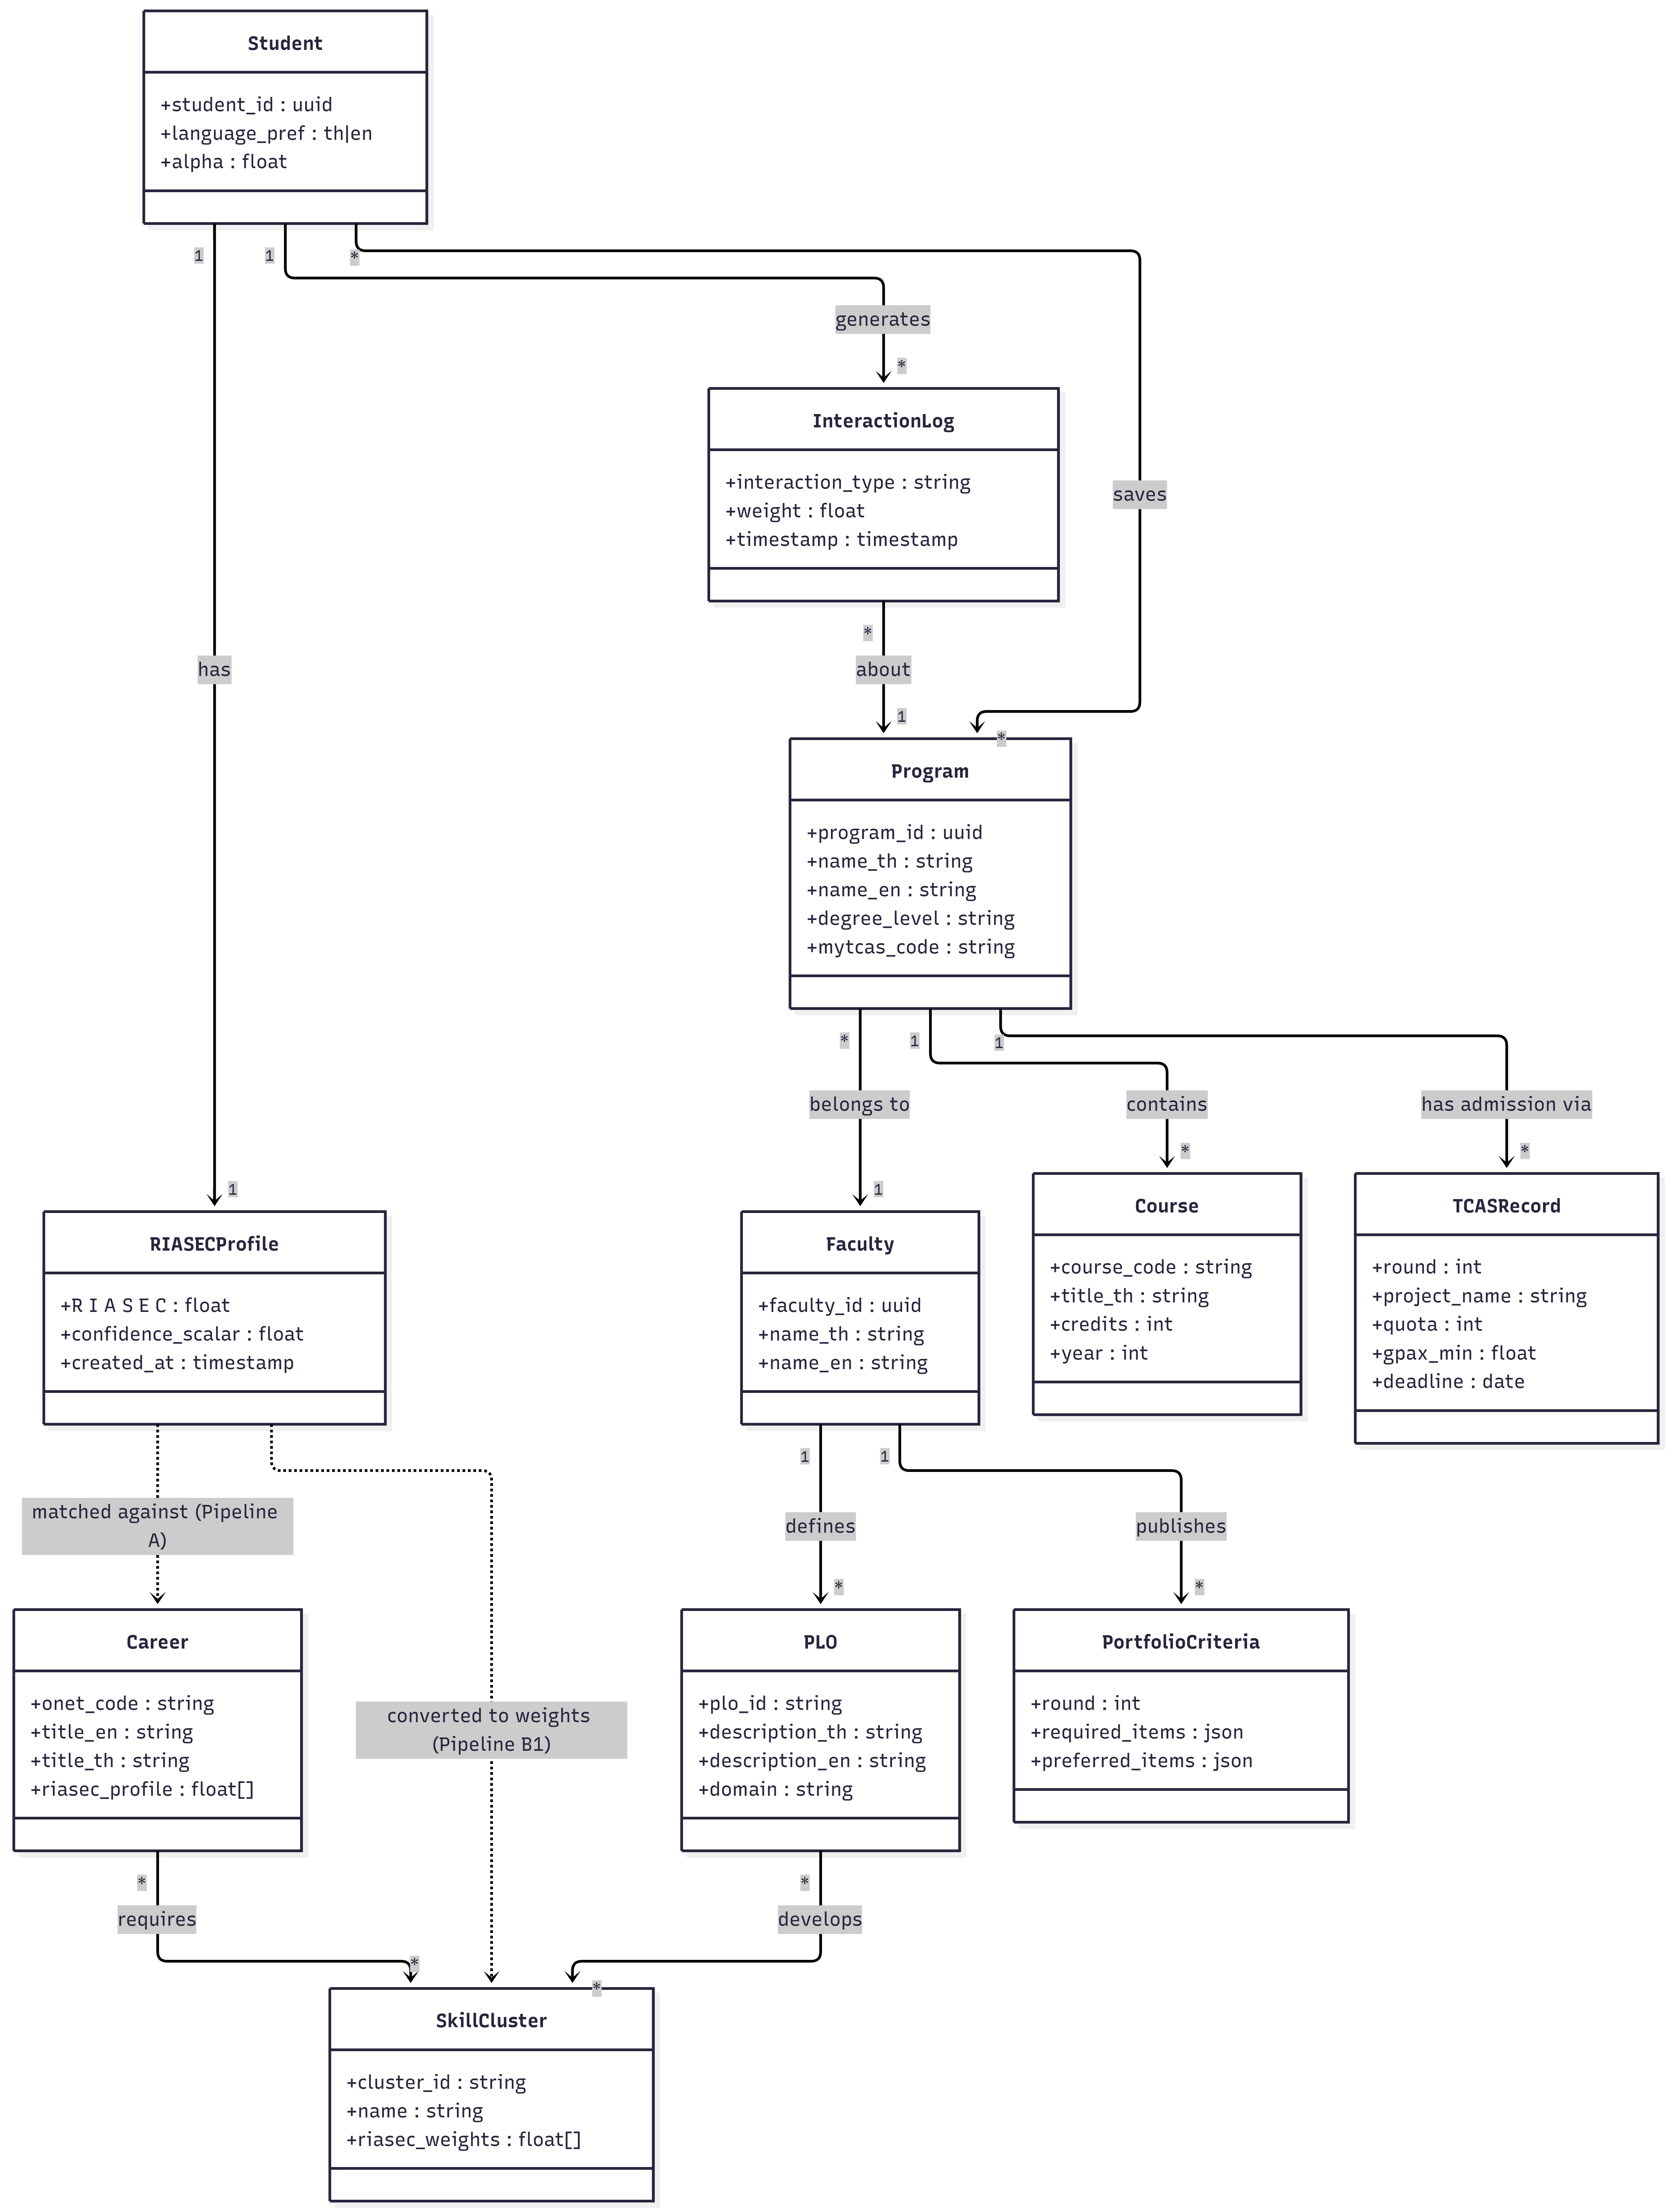
\includegraphics[width=\textwidth]{diagrams/domain-model.png}
    \caption{KUru Domain Model}
    \label{fig:domain-model}
\end{figure}

\section{Software Design}
\label{section:software-design}

\subsection{RAG Pipeline Sequence}
\label{subsection:rag-pipeline}

When a user submits a query to the curriculum chatbot: (1) the query is embedded locally using \texttt{intfloat/multilingual-e5-base}; (2) the embedding is used to perform a cosine similarity search against the pgvector store of มคอ.2 document chunks; (3) the top-$k$ retrieved chunks are assembled into a prompt context along with the user query and the conversation history; (4) Gemini 2.5 Flash Lite via OpenRouter generates a grounded response in the requested language; (5) source citations are appended to the response. In the current POC, citation chips expose provenance such as source file, section type, and similarity/confidence context, but they do not yet open the exact PDF page or extracted chunk. Deep source inspection is Phase~2; the future API should include \texttt{chunk\_id}, page number, and source URL so the frontend can open a source preview panel or PDF page.

\begin{figure}[p]
    \centering
    
\includegraphics[width=\textwidth]{diagrams/rag-pipeline.png}
    \caption{RAG Pipeline Sequence}
    \label{fig:rag-pipeline}
\end{figure}

\subsection{Recommendation Pipeline Sequence}
\label{subsection:recommendation-pipeline}

For the evaluated MVP, recommendation uses the simplified Pipeline~B2 path. RIASEC is not treated as proof that a student will be satisfied with a program after graduation. Instead, it is used as an interest signal that can be converted into curriculum search intent. When a student completes the interest discovery flow, the backend converts the RIASEC profile into interest themes and a semantic query, retrieves semantically similar program/PLO/course chunks from Supabase pgvector, aggregates evidence by program, computes a curriculum-fit score, and generates a cited plain-language explanation from the retrieved evidence. This is the recommendation behaviour evaluated for MVP pass/fail.

For example, a high Investigative--Realistic profile is converted into themes such as analysis, problem solving, systems, technical design, experiments, and hands-on laboratory work. These themes are embedded as a semantic query and matched against curriculum evidence such as PLOs, course descriptions, project-based learning statements, laboratory requirements, and technical skill outcomes. A program ranks highly only when retrieved curriculum chunks support the match.

\begin{figure}[htbp]
    \centering
    \fbox{\parbox{0.92\textwidth}{
    \textbf{MVP recommendation flow:}
    RIASEC answers $\rightarrow$ 6D RIASEC profile $\rightarrow$ top dimensions / Holland code $\rightarrow$ interest themes and semantic query $\rightarrow$ Supabase/pgvector search over program, PLO, and course chunks $\rightarrow$ group evidence by program $\rightarrow$ curriculum-fit score $\rightarrow$ ranked programs with evidence-grounded explanation.
    }}
    \caption{MVP Recommendation Pipeline: RIASEC-to-Curriculum Semantic Matching}
    \label{fig:mvp-recommendation-pipeline}
\end{figure}

The full target-system recommendation pipeline proceeds in five stages using two independent parallel signals:

\begin{enumerate}[leftmargin=80pt]
    \item \textbf{RIASEC vector construction.} The twelve-step adaptive elicitation (UC-01) produces a weighted 6-dimensional RIASEC vector. Steps~1--6 (Likert screens) produce raw scores per dimension (max 20 each). Step~7 applies a global confidence scalar (1.0, 0.75, or 0.5). Step~8 (adaptive pairwise) adjusts scores for dimension pairs with delta $< 3$. Steps~9--11 (scenario questions) adjust scores proportionally per response. Step~12 applies the optional dealbreaker filter, zeroing out explicitly rejected dimensions. The resulting vector is L2-normalised to a unit vector. The MVP uses this vector to form a Pipeline~B2 curriculum search intent; the target system also uses it in Pipeline~A and Neo4j Pipeline~B1.

    \item \textbf{Parallel signal computation.} Two independent pipelines run concurrently:

    \textbf{Pipeline A (Career-side):} The student RIASEC vector is compared against precomputed O*NET occupation RIASEC interest profiles in Supabase pgvector using cosine similarity. O*NET interest profiles are empirically derived from surveys of employed workers, making this step grounded in real-world data. The top 10--15 occupations form the internal career space; the top 7 are surfaced to the student in the Career Explorer (UC-06). An A-score per KU program is computed based on career-program pathway alignment. O*NET's 35-skill taxonomy is used for Career Explorer display in UC-06 only --- it is not used as a bridge to Neo4j in the ranking pipeline.

    \textbf{Pipeline B (Curriculum-side):} Two sub-signals computed independently and combined:
    \begin{itemize}[leftmargin=40pt]
        \item \textbf{B1 --- Neo4j PLO match:} The student's RIASEC vector is converted to a SkillCluster weight vector and matched against KU program PLO SkillCluster profiles via Neo4j graph query. B1-score is the cosine similarity between the student weight vector and each program's PLO skill profile.
        \item \textbf{B2 --- Semantic course content match:} The student's interest query is matched against course description embeddings in Supabase pgvector via semantic search over ingested มคอ.2 course content. B2-score is the weighted mean similarity of the top retrieved course chunks per program.
    \end{itemize}
    Combined B-score $= 0.4 \times \text{B1} + 0.6 \times \text{B2}$.

    The two pipelines are independent --- an error in Pipeline~A does not propagate into Pipeline~B.

    \item \textbf{Score synthesis.} Programs are ranked by a final score combining both pipeline outputs:
    \[\text{score} = 0.35 \times \text{A-score} + 0.65 \times \text{B-score}\]
    The top-$N$ programs are selected for display.

    \item \textbf{Explanation generation.} The top-$N$ ranked programs, together with their Pipeline~A details (matched O*NET occupations) and Pipeline~B details (curriculum themes and matched PLOs), are passed to Gemini 2.5 Flash as structured context. Gemini generates a plain-language explanation for each program referencing both career alignment and curriculum fit. Explanations are generated in Thai or English depending on the student's language setting.

    \item \textbf{Behavioural re-ranking (registered users only).} For registered users with accumulated interaction data, the pipeline scores from Stage~3 are blended with a behavioural fit score derived from the individual student's own interaction history (not from other users --- true collaborative filtering across students is deferred to Phase~2). The blend ratio is controlled by $\alpha$: new users start at $\alpha = 1.0$ (pure pipeline score); $\alpha$ decays toward 0.2 as interaction weight accumulates according to the threshold schedule documented in UC-07 (3--5 meaningful signals $\rightarrow$ $\alpha \approx 0.5$; regular user $\rightarrow$ $\alpha \approx 0.2$). The final ranking score is:
    \[\text{final score} = \alpha \times \text{pipeline score} + (1 - \alpha) \times \text{behavioural fit}\]
    Guest interaction signals are session-scoped and do not update $\alpha$; guests always begin a new session at $\alpha = 1.0$. Fallback hierarchy when behavioural data is sparse: (1) sufficient interaction history $\rightarrow$ normal blended signal; (2) limited interaction history $\rightarrow$ $\alpha$ held higher; (3) no interaction history $\rightarrow$ pure pipeline score ($\alpha = 1.0$). Interaction weights are documented in UC-07.
\end{enumerate}

\begin{figure}[p]
    \centering
    
\includegraphics[height=0.9\textheight, keepaspectratio]{diagrams/recommendation-pipeline.png}
    \caption{Phase~2 Target-System Recommendation Pipeline --- Five Stages with Two Parallel Signals}
    \label{fig:recommendation-pipeline}
\end{figure}

\subsection{Interest Elicitation Flow}
\label{subsection:elicitation-flow}

The interest elicitation flow (UC-01) produces the RIASEC vector that seeds the MVP recommendation pipeline. In Phase~2, the same vector can also seed the Career Explorer. The flow is adaptive: the pairwise comparison step (Step~8) is shown only when at least one dimension pair has a score delta below the 3-point ambiguity threshold; students with a clearly differentiated Likert profile skip directly to the scenario questions. Figure~\ref{fig:elicitation-flow} shows the full conditional logic from entry to RIASEC vector output.

\begin{figure}[p]
    \centering
    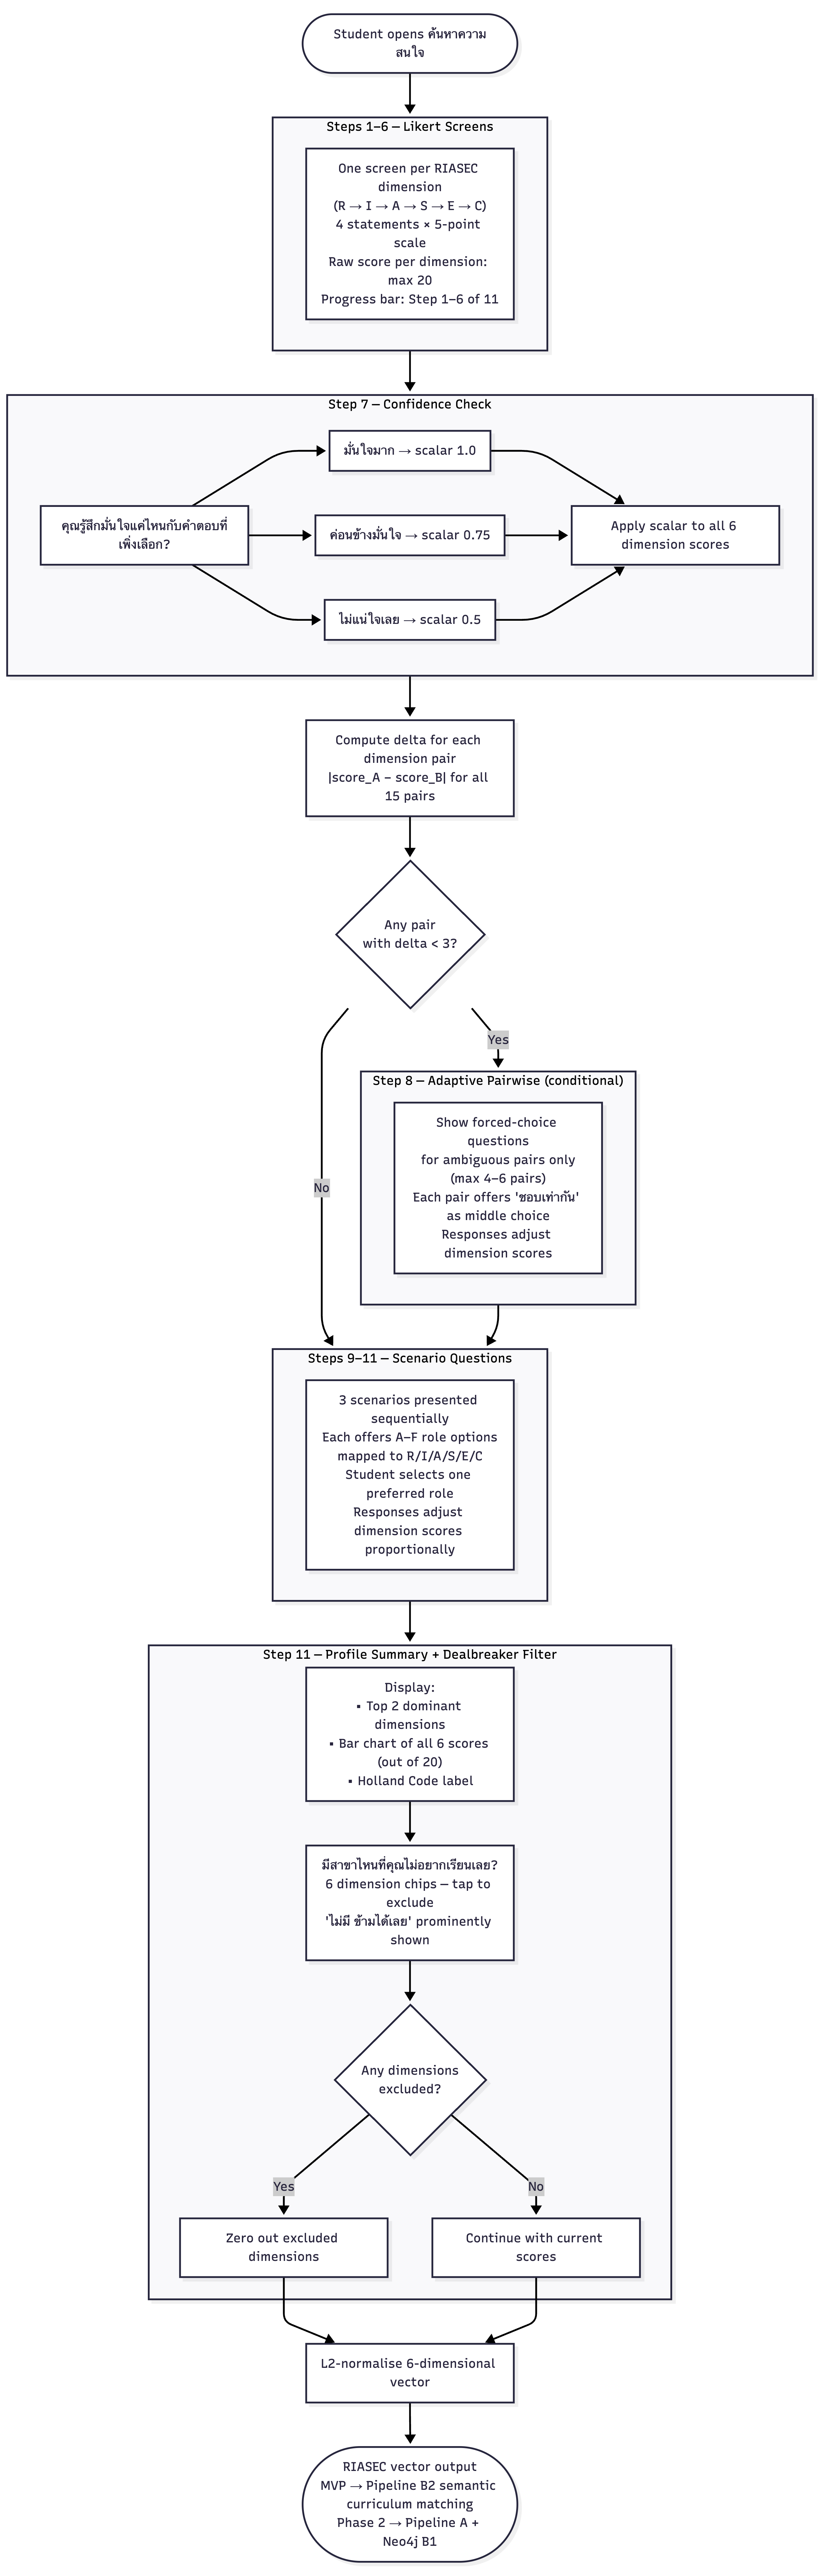
\includegraphics[height=0.9\textheight, keepaspectratio]{diagrams/elicitation-flow.png}
    \caption{Interest Elicitation Flow (UC-01) — 12-Step Adaptive Process}
    \label{fig:elicitation-flow}
\end{figure}

\section{AI and Data Design}
\label{section:ai-data-design}

\subsection{Data Sources and Collection}
\label{subsection:data-sources}

\begin{itemize}[leftmargin=80pt]
    \item \textbf{KU curriculum documents (มคอ.2):} Provided directly by KU faculty advisors for all KU programs. Thai-language PDFs of varying length (typically 20--80 pages per program). These are the primary knowledge base for both the RAG pipeline and the PLO extraction pipeline. Documents are version-tagged by academic year and re-ingested when updated.

    \item \textbf{O*NET occupational database \cite{onet2024}:} Publicly available from the US Department of Labor. Contains two data layers used by KUru: (a) \textit{Interests} --- the RIASEC profile for each occupation, derived from surveys of employed workers, used for career matching from the student's RIASEC vector; and (b) \textit{Skills} --- 35 standardized skills per occupation with importance and level scores, displayed in the Career Explorer (UC-06) to show students what skills their matched careers require. Not used as a bridge to Neo4j in the ranking pipeline --- Pipeline~B1 queries Neo4j directly from the RIASEC-derived SkillCluster weight vector. Downloaded as structured data (CSV/JSON). Occupation titles are mapped to Thai equivalents for student-facing display; skill and interest data are used directly as the underlying structure is language-independent.

    \item \textbf{TCAS admission data:} Ingested from three sources in priority order. (1)~\textit{KU faculty-provided project PDFs} received via Google Drive --- each PDF (e.g., โครงการช้างเผือก.pdf) may contain admission records for multiple programs across multiple faculties. A batch downloader retrieves all PDFs recursively. Each PDF is classified as tcas / mko2 / portfolio / unknown using rule-based keyword detection on the first page. TCAS PDFs are processed by a structured extraction pipeline using Gemini to parse per-program TCASRecord objects covering project name, round, faculty, program name, quota, GPAX minimum, exam score criteria, portfolio requirements, and application deadlines. (2)~\textit{mytcas.com} --- scraped as a gap-filling layer for programs not covered by faculty PDFs, using the mytcas\_code field in the canonical program registry. (3)~\textit{Faculty portfolio criteria PDFs} --- retained as a Phase~2 source for the Portfolio Readiness Checker rather than an MVP pass/fail requirement. Available sources are resolved against a canonical program registry using fuzzy name matching with PyThaiNLP normalization and sequence similarity scoring (threshold 0.85). Records below this threshold are flagged for manual review. A Supabase materialized view (\texttt{programs\_unified}) joins มคอ.2 structured data, TCAS records, and available admission metadata into a unified program record keyed on program\_id, refreshed after each ingestion run.

    \item \textbf{Interaction log (Phase~2):} Generated by the system as registered users engage with KUru. Stored in Supabase PostgreSQL. Records program saves, card expansions, TCAS guide views, chatbot queries, and card views, each with a timestamp, interaction weight, and associated program identifier. Used to compute the behavioural fit score in Stage~5 of the target-system recommendation pipeline. Not required for MVP pass/fail evaluation.

    \item \textbf{Faculty portfolio criteria documents (Phase~2):} Published by KU faculties for TCAS Round~1 and Round~2 applications. Ingested via the same PDF extraction pipeline as มคอ.2 using Gemini in structured extraction mode to produce a per-faculty, per-round criteria schema. Stored in Supabase PostgreSQL alongside TCAS admission data. Updated at the start of each TCAS cycle. Used by the Portfolio Readiness Checker.

    \item \textbf{Course structure data (partial MVP / Phase~2):} Extracted from มคอ.2 during ingestion as a structured layer stored separately from the embedding chunks where available. MVP uses available course and PLO text for RAG, semantic search, and simplified recommendation. Full per-year course timeline visualisation is Phase~2.
\end{itemize}

มคอ.2 document ingestion uses a six-stage pipeline:

\begin{enumerate}[leftmargin=80pt]
    \item \textbf{PDF classification.} Pages are classified by text density and Thai character density (minimum 20\% Thai Unicode characters for Thai-language documents, minimum 100 characters per page) into born-digital, scanned, pure-image, or mixed types.

    \item \textbf{Tiered text extraction.} The current curriculum ingestion pipeline first runs PyMuPDF on every PDF page. Pages with very low text yield are rendered to images and sent to Typhoon OCR (\texttt{typhoon-ocr}) when \texttt{TYPHOON\_API\_KEY} is available; recent targeted re-ingests mostly record \texttt{pymupdf+typhoon\_pages}. If the whole PDF remains below the scanned-document threshold, the ingest script treats it as a full scanned PDF and calls the isolated \texttt{ocr\_extractor.extract\_with\_ocr()} path. That full scanned-PDF path uses the configured \texttt{OCR\_MODEL}: by default direct Gemini \texttt{gemini-2.5-flash}, or Typhoon/OpenRouter if explicitly configured, with Tesseract as a last local fallback when vision OCR yields too little text. Each page is tagged with its extraction method (\texttt{pymupdf}, \texttt{typhoon\_page}, \texttt{scanned}, or \texttt{gemini\_ocr}) for coverage reporting.

    \item \textbf{Section-aware chunking.} PLO sections, course descriptions, admission requirements, and curriculum structure sections are chunked separately (target 500 tokens, 50-token overlap) to preserve semantic coherence. Each chunk is tagged with section type (\texttt{plo} / \texttt{course} / \texttt{admission} / \texttt{curriculum\_structure} / \texttt{general}).

    \item \textbf{Structured extraction.} After text extraction and chunking, Gemini text mode (\texttt{LLM\_MODEL=gemini-2.5-flash-lite} by default) extracts program metadata, PLOs, course lists, year timeline fields, and curriculum mapping into structured JSON. The MVP stores these fields in Supabase for program detail pages, semantic search, RAG grounding, and coverage reporting. Neo4j population from PLO/skill data is Phase~2.

    \item \textbf{Embedding generation.} The current POC uses the local multilingual E5 embedding model (\texttt{intfloat/multilingual-e5-base}) to embed chunks before upserting them to Supabase/pgvector. This avoids external embedding quota limits. Chunks from failed OCR pages are excluded.

    \item \textbf{Target-system graph population and quality reporting.} For Phase~2, Program $\rightarrow$ PLO $\rightarrow$ SkillCluster nodes and edges are created in Neo4j from the structured PLO extraction output. For the MVP, the corresponding quality report focuses on whether curriculum, TCAS, fee, and PLO chunks are retrievable from Supabase/pgvector and whether documents with OCR or extraction failures are flagged for manual review.
\end{enumerate}

\subsection{Model Design}
\label{subsection:model-design}

The primary answer-generation model for the MVP RAG path is Gemini 2.5 Flash Lite via OpenRouter, selected for Thai/English response quality and cost efficiency. Direct Gemini text-mode calls are used for structured extraction where appropriate, and direct Gemini vision OCR is used only in the isolated full scanned-PDF OCR path when configured. The project avoids LangChain or similar orchestration frameworks to reduce latency and maintain explicit control over prompt structure.

Embeddings use the local \texttt{intfloat/multilingual-e5-base} model, with the query/passage prefixes required by the E5 family. This model produces multilingual semantic representations for Thai and English while avoiding Gemini embedding quota limits.

The Phase~2 Neo4j knowledge graph uses a schema with four node types: Faculty, PLO, SkillCluster, and Career. Edges represent: Faculty -[HAS\_PLO]$\rightarrow$ PLO, PLO -[DEVELOPS]$\rightarrow$ SkillCluster, Career -[REQUIRES]$\rightarrow$ SkillCluster. This schema supports the multi-hop queries required for the target-system recommendation: given a student's SkillCluster profile, find Faculties whose PLOs develop those clusters.

The interest discovery interface uses a 12-step elicitation flow grounded in Holland's RIASEC model \cite{holland1997}. Steps~1--6 present one RIASEC dimension per screen with 4 Likert statements each (5-point scale, max score 20 per dimension). Step~7 applies a global confidence scalar (1.0 / 0.75 / 0.5) to all dimension scores based on a single self-reported confidence question. Step~8 presents adaptive pairwise forced-choice questions targeting only dimension pairs where the score delta is below a 3-point threshold, with a maximum of 4--6 pairs shown. Steps~9--11 present three scenario questions with A--F role options mapped to RIASEC dimensions, adjusting scores proportionally. Step~12 displays the profile summary with an optional dealbreaker filter that zeros out any explicitly rejected dimensions before L2-normalisation. The full question bank is documented in Appendix~\ref{appendix:A}.

The MVP recommendation ranking uses Pipeline~B2 curriculum-side semantic fit only. The Phase~2 target ranking blends the RIASEC-derived fit score with a behavioural fit score using a blending weight $\alpha$ that decays automatically as the student accumulates interaction data: new users start at $\alpha = 1.0$ (pure RIASEC); after 3--5 meaningful interactions $\alpha \approx 0.5$ (balanced blend); regular users converge toward $\alpha \approx 0.2$ (behaviour-dominated). Interaction signals are weighted by type: program save (1.0), TCAS guide viewed (0.8), chatbot query about a program (0.6), card expanded (0.4), card viewed (0.1).

The baseline for comparison is keyword-only \texttt{ilike} search over the same มคอ.2 corpus without embedding-based retrieval or LLM generation. The full RIASEC-to-topic mapping is documented in Appendix~\ref{appendix:A}.

\subsection{Evaluation}
\label{subsection:evaluation}

\begin{itemize}[leftmargin=80pt]
    \item \textbf{Current POC baseline (May~2026):} The current RAG POC is evaluated with custom LLM-as-judge regression tests tracked in MLflow on a 0--3 scale, including TCAS, fee, alias, bilingual, and missing-data honesty checks. The selected production regression run, \texttt{v8\_structured\_tcas\_fees}, records 72.7\% good answers and an average score of 2.055/3.0 on the fee/TCAS regression suite. The headline retrieval benchmark, \texttt{latest\_submission\_headline\_v7\_rerank\_74pct}, records 74\% good answers and an average score of 2.26/3.0. RAGAS was considered but is not the primary POC metric because custom checks better capture Thai/English KU-specific correctness, structured TCAS/fee evidence, and missing-data honesty. This baseline is reported honestly as POC evidence, not as final MVP success.

    \item \textbf{Final MVP RAG quality:} RAGAS framework metrics \cite{es2023ragas} are added as standardized supplementary metrics for UC-04 and UC-08: Faithfulness (proportion of claims in the answer supported by retrieved context), Answer Relevancy (semantic similarity between answer and question), and Context Recall (proportion of relevant information retrieved). Target: Faithfulness $>$ 0.80, Answer Relevancy $>$ 0.75. Custom regression tests remain required for TCAS, fees, aliases, bilingual behaviour, and missing-data honesty because these behaviours are KU-specific.

    \item \textbf{Recommendation quality:} The MVP does not claim to measure whether a student will remain satisfied with a selected program after four years. That outcome is longitudinal and cannot be observed within the project period. Instead, recommendation quality is evaluated as a short-term relevance and explainability task: given a manually curated set of 30--50 student interest profiles, the system must rank programs judged relevant by faculty advisors, senior students, or documented curriculum evidence. Metrics are Mean Reciprocal Rank (MRR) and NDCG@5, with target MRR $>$ 0.60. Explanations are also checked for faithfulness to the retrieved curriculum evidence. The MVP evaluates the simplified Pipeline~B2 recommender; career-path validation, full hybrid Pipeline~A+B, and Neo4j B1 evaluation are Phase~2.

    \item \textbf{Interest discovery and semantic search usability:} UC-01 completion rate target $>$ 80\%, with System Usability Scale (SUS) score from user testing with 10--15 high school students or KU first-year students. UC-09 is evaluated through semantic query checks and user task completion. Target: SUS score $>$ 70 (acceptable).
\end{itemize}

    \chapter{Software Development}
\label{chap:software-development}

%% PROPOSAL: Sections 5.1-5.3 hidden for proposal, showing only Schedule (5.4)

%% \section{Software Development Methodology}
%% \label{section:software-development-methodology}
%% 
%% The project uses an Agile-inspired iterative approach adapted for a two-person team over one semester. Development is organized into two-week sprints aligned with the phases in the project schedule. Each sprint ends with a working, demonstrable increment. A shared Kanban board (Notion) tracks tasks, and GitHub is used for version control with a feature-branch workflow. Weekly check-ins with the project advisor provide feedback and course correction.
%% 
%% Given the data dependency at the start of the project (มคอ.2 documents from faculty), the first two weeks are allocated to data collection and pipeline setup, with feature development beginning only once the core data layer is operational.

%% \section{Technology Stack}
%% \label{section:technology-stack}

%% \begin{itemize}[leftmargin=80pt]
%%     \item \textbf{Frontend:} Next.js 14 (App Router), Tailwind CSS, Shadcn/UI. Chosen for familiarity, strong TypeScript support, and built-in i18n routing for Thai/English.
%% 
%%     \item \textbf{Backend:} Python FastAPI. Chosen for Python ecosystem access (PyMuPDF for PDF processing, sentence-transformers, neo4j driver) and async performance.
%% 
%%     \item \textbf{Vector database:} Supabase (PostgreSQL + pgvector extension). Stores มคอ.2 document embeddings, precomputed O*NET occupation interest profiles, user profiles, TCAS structured data, and the interaction log (program saves, card views, TCAS guide views, chatbot queries with weights and timestamps). A background job periodically recomputes collaborative scores from the interaction log. Supabase Auth handles authentication.
%% 
%%     \item \textbf{Graph database:} Neo4j on Railway. Stores the PLO--Skill--Career knowledge graph. Queried via Cypher from the FastAPI backend.
%% 
%%     \item \textbf{AI:} Gemini 2.5 Flash Lite via OpenRouter for generation, local multilingual-E5 for embeddings, Gemini text mode for structured extraction.
%% 
%%     \item \textbf{Data processing:} PyMuPDF for page text extraction, Typhoon OCR via opentyphoon.ai for low-yield pages, isolated full scanned-PDF OCR through the configured OCR model when needed, local multilingual-E5 embeddings, Gemini text-mode structured extraction, and custom Python chunking.
%% 
%%     \item \textbf{Thai NLP:} PyThaiNLP --- Thai text normalization used in TCAS program name entity resolution (fuzzy matching with sequence similarity scoring).
%% 
%%     \item \textbf{Deployment:} Vercel (frontend), Railway (FastAPI backend + Neo4j).
%% \end{itemize}
%% 
%% \section{Coding Standards}
%% \label{section:coding-standards}
%% 
%% \begin{itemize}[leftmargin=80pt]
%%     \item \textbf{Python:} PEP 8, type hints on all function signatures, docstrings for all public functions.
%% 
%%     \item \textbf{TypeScript:} ESLint with Next.js recommended config, Prettier for formatting.
%% 
%%     \item \textbf{Git:} Conventional commits format (feat/fix/chore/docs). Feature branches merged via pull request with at least one review.
%% 
%%     \item \textbf{Environment:} All secrets managed via .env files, never committed. Supabase and Gemini API keys stored as environment variables.
%% \end{itemize}

\section{Schedule}
\label{section:schedule}

Development is organized into four phases across April~2026 and January--March~2027. P1~Foundation runs April~1--12, P2~Core~AI POC runs April~6--30, P3~MVP Feature Completion runs January~2027, and P4~Polish \& Evaluation runs February--March~2027. By the end of April~2026, the current proof of concept demonstrates the data ingestion pipeline, grounded RAG chatbot, and Program Explorer over indexed curriculum content. Recommendation, explanation, and PLO/profile visualisation remain MVP features to be completed and evaluated during P3--P4.

\begin{table}[htbp]
\centering
\footnotesize
\renewcommand{\arraystretch}{1.4}
\caption{Project Schedule}
\label{tab:schedule}
\begin{tabularx}{\textwidth}{|L{3cm}|L{3.2cm}|Y|}
\hline
\textbf{Period} & \textbf{Phase} & \textbf{Deliverables} \\
\hline
Apr 1--5, 2026 & P1 · Foundation — Set up Repo & Repository setup, project structure, development environment \\
\hline
Apr 1--5, 2026 & P1 · Foundation — Data Collection & Receive มคอ.2 and TCAS admission data from KU faculty, download O*NET dataset \\
\hline
Apr 6--12, 2026 & P1 · Foundation — Data Ingestion & PDF extraction, chunking, embedding into Supabase pgvector; graph schema exploration for Phase~2 \\
\hline
Apr 6--30, 2026 & P2 · Core AI POC — RAG Chatbot & RAG pipeline over indexed curriculum and TCAS/fee data, grounded answer generation, source citations \\
\hline
Apr 6--30, 2026 & P2 · Core AI POC — Program Explorer & Semantic search and browsing over indexed program content and metadata using Supabase/pgvector \\
\hline
Apr 6--30, 2026 & P2 · Core AI POC — Demo Integration & Working proof-of-concept demo combining ingestion output, Program Explorer, and RAG chatbot \\
\hline
Jan 1--31, 2027 & P3 · MVP Features — Interest Discovery & RIASEC elicitation flow, profile scoring, confidence adjustment, and profile summary \\
\hline
Jan 1--31, 2027 & P3 · MVP Features — Program Detail Pages & Program detail pages, static PLO/profile chart, and available TCAS information \\
\hline
Jan 1--31, 2027 & P3 · Phase~2 Prototype — Portfolio Coach & Optional prototype UI only; excluded from MVP pass/fail evaluation \\
\hline
Jan 31, 2027 & P3 · MVP Features — Complete Recommendation & Complete simplified Pipeline~B2 recommendation, evidence-grounded explanation, and Program Explorer refinement \\
\hline
Feb 1--28, 2027 & P4 · Polish \& Eval — UI/UX Polish & UI/UX polish, Thai/English language switching, mobile-first refinement \\
\hline
Feb 1--28, 2027 & P4 · Polish \& Eval — Cross-feature Integration & Chatbot + Explorer + Recommendation + Program Detail integration \\
\hline
Feb 1--28, 2027 & P4 · Polish \& Eval — User Testing & RAGAS plus custom TCAS/fee regression, MRR/NDCG test set, SUS user testing with 10--15 students \\
\hline
Mar 1--31, 2027 & P4 · Polish \& Eval — Performance Testing & Performance benchmarking against all success metric targets \\
\hline
Mar 1--31, 2027 & P4 · Polish \& Eval — Bug Fixing \& Optimization & Bug fixes, optimization, stability improvements \\
\hline
Mar 1--31, 2027 & P4 · Polish \& Eval — Final Documentation & Final report, demo preparation, project documentation \\
\hline
\end{tabularx}
\end{table}

%% PROPOSAL: Progress Tracking Report hidden
%% \section{Progress Tracking Report}
%% \label{section:progress-tracking-report}
%% 
%% \begin{figure}[h]
%%     \centering
%%     \fbox{\parbox{0.9\textwidth}{\centering\vspace{1em}
%%     \textit{[GitHub contribution graph and sprint burndown charts to be included here as the project progresses.]}
%%     \vspace{1em}}}
%%     \caption{Progress Tracking}
%%     \label{fig:progress-tracking}
%% \end{figure}

    %% PROPOSAL: Deliverables, Discussion hidden
    %% \chapter{Deliverables}
\label{chap:deliverable}

\section{Software Solution}
\label{section:software-solution}

\begin{figure}[h]
    \centering
    \fbox{\parbox{0.9\textwidth}{\centering\vspace{1em}
    \textit{[GitHub repository link to be added. Screenshots of each application screen to be included upon completion.]}
    \vspace{1em}}}
    \caption{Application Screenshots}
    \label{fig:app-screenshots}
\end{figure}

The delivered software will include: a deployed web application accessible at a public URL; the data ingestion pipeline for มคอ.2 PDF processing; the Neo4j knowledge graph populated with all KU programs; the RAG pipeline and recommendation engine; and the six core MVP features described in Chapter~\ref{chap:introduction}.

\section{Test Report}
\label{section:test-report}

Testing will cover three levels:

\begin{itemize}[leftmargin=80pt]
    \item \textbf{Unit tests:} Core AI functions (chunking, embedding, retrieval, graph query) tested with pytest. Coverage target: 70\% of backend functions.

    \item \textbf{Integration tests:} End-to-end API tests for each major user flow (interest discovery to recommendation, chatbot query to grounded response). Run automatically on each pull request via GitHub Actions.

    \item \textbf{User tests:} Manual usability testing sessions with 10--15 participants, using a structured task script and SUS questionnaire. Results tabulated and reported in the test report.
\end{itemize}

    %% \chapter{Conclusion and Discussion}
\label{chap:conclusion-discussion}

\section{Summary of Achievements}
\label{section:summary-of-achievements}

\begin{figure}[h]
    \centering
    \fbox{\parbox{0.9\textwidth}{\centering\vspace{1em}
    \textit{[To be completed at project conclusion. Will summarize delivered features, evaluation results, and degree to which the problem statement was addressed.]}
    \vspace{1em}}}
    \caption{Summary placeholder}
    \label{fig:summary-placeholder}
\end{figure}

\section{Known Limitations}
\label{section:limitations}

\begin{itemize}[leftmargin=80pt]
    \item \textbf{TCAS data currency:} TCAS admission requirements change each academic year. The system requires manual data updates at the start of each TCAS cycle and does not automatically detect changes.

    \item \textbf{CLO-level mapping:} The system uses program-level PLO data (มคอ.2) only. Course-level CLO data (มคอ.3) is not ingested, as features requiring CLO mapping (e.g., skill progress tracking for enrolled students) are out of scope for this project.

    \item \textbf{O*NET Thai career mapping:} O*NET occupational data is in English and uses US career taxonomy. Manual mapping to Thai career titles and KU graduate employment patterns is required and introduces approximation.

    \item \textbf{Portfolio scorer:} Designed and documented but not implemented in the MVP due to data dependency on structured per-faculty portfolio rubrics from the admissions office.

    \item \textbf{Evaluation ground truth:} The MRR evaluation test set is manually curated with limited size (30--50 profiles), which constrains the statistical reliability of the recommendation quality metrics.

    \item \textbf{Interest profile validity:} The interest discovery interface uses a five-step adaptive elicitation process as a lightweight proxy for established vocational interest instruments such as Holland's Self-Directed Search. While the five-step design is substantially more reliable than a two-question approach, it remains shorter than a full validated instrument (42+ items for the Self-Directed Search). Meta-analytic research on validated interest inventories reports approximately 50\% accuracy in predicting eventual career choice even with full assessments; the accuracy of KUru's abbreviated elicitation is expected to be lower. The system is designed accordingly --- recommendations are framed as a starting point for exploration rather than a definitive match, with the $\alpha$ blending mechanism progressively shifting recommendation weight toward behavioural signals as the student interacts with the system.

    \item \textbf{Behavioural blending cold start:} The $\alpha$ blending mechanism that combines RIASEC fit scores with behavioural fit scores provides no benefit until sufficient interaction data has accumulated. For early users of the system, collaborative signal is sparse or absent, and the system falls back toward pure RIASEC recommendations. The fallback hierarchy is: (1) sufficient similar-profile users exist $\rightarrow$ collaborative signal applied normally; (2) few similar users $\rightarrow$ $\alpha$ is held higher regardless of individual interaction count; (3) no similar users $\rightarrow$ pure RIASEC ($\alpha = 1.0$). Logged-in users always receive better personalisation than guests, as guest interaction signals are session-scoped and do not persist.
\end{itemize}

\section{Future Work}
\label{section:future-work}

\begin{itemize}[leftmargin=80pt]
    \item \textbf{KU enrolled student features (Phase 2):} Once the pre-admission system is validated, extend scope to serve currently enrolled KU students. This would require มคอ.3 CLO ingestion, a course enrollment interface, and a skill gap dashboard. The current knowledge graph schema is designed to support this extension without architectural changes.

    \item \textbf{Portfolio scorer:} Build the AI-assisted portfolio evaluation feature once structured admission rubrics are available from the KU admissions office.

    \item \textbf{Automated TCAS data refresh:} Monitor mytcas.com for changes each TCAS cycle and automatically notify the data administrator when updates are detected, triggering a review and re-ingestion cycle with KU faculty.

    \item \textbf{Thai career taxonomy alignment:} Develop a systematic mapping between O*NET occupations and THACO (Thai Standard Occupational Classification) to improve career recommendation accuracy for Thai students.

    \item \textbf{True collaborative filtering (Phase 2):} The current MVP implements single-user behavioural blending --- the $\alpha$ mechanism in UC-07 weights each student's \textit{own} interaction history against their initial RIASEC scores. True collaborative filtering --- using interaction patterns of students with similar RIASEC profiles to inform each other's recommendations --- requires a critical mass of user data and is deferred to Phase~2. The $\alpha$ integration point in Stage~6 of the recommendation pipeline is designed to accommodate this extension without architectural changes. A prerequisite is robust handling of \textit{profile pollution}: a poor initial RIASEC vector clusters a student incorrectly, degrading the collaborative signal for all students in that cluster. The five-step adaptive elicitation in UC-01 is designed to reduce this risk before true collaborative filtering is introduced.

    \item \textbf{Longitudinal evaluation:} Track recommendation quality by following up with admitted students after one year to assess whether their actual program experience matched the system's prediction.
\end{itemize}

    %% Chapters section

    \input{common/onetextpage.tex}
    \onetextpage{Reference}
    \bibliographystyle{IEEEtran}
    \bibliography{bibliography}

    \input{common/onetextpage.tex}
\newcounter{nappendix}
\renewcommand{\thenappendix}{\Alph{nappendix}}
\newcommand{\newappendix}[1]{%
    \refstepcounter{nappendix}
    \onetextpage{Appendix \thenappendix}
    \chapter*{Appendix \thenappendix: #1}
    \label{appendix:\thenappendix}
    \addcontentsline{toc}{chapter}{Appendix \thenappendix: #1}
}

%% Edit past this comment line.

\newappendix{RIASEC-to-Topic Cluster Mapping}

\setcounter{table}{0}
\renewcommand{\thetable}{A.\arabic{table}}

Table~\ref{tab:riasec-mapping} documents the mapping between Holland's six RIASEC types and the eight topic clusters presented in the interest discovery interface. Each topic tile is assigned a primary RIASEC type and a secondary RIASEC type with associated weights. When a student selects a tile, both weights are added to the corresponding dimensions of the 6-dimensional RIASEC vector. After all five elicitation steps (tile selection, pairwise comparisons, scenario confirmation, dealbreaker filter, and confidence weighting), the vector is L2-normalised before use in retrieval and fit score computation.

\begin{table}[htbp]
\centering
\small
\renewcommand{\arraystretch}{1.4}
\caption{RIASEC-to-Topic Cluster Weight Mapping}
\label{tab:riasec-mapping}
\begin{tabularx}{\textwidth}{|p{3.5cm}|p{2.5cm}|p{1.2cm}|p{3cm}|p{1.2cm}|}
\hline
\textbf{Topic Cluster} & \textbf{Primary RIASEC} & \textbf{Weight} & \textbf{Secondary RIASEC} & \textbf{Weight} \\
\hline
Computers \& Digital & Investigative (I) & 0.8 & Realistic (R) & 0.5 \\
\hline
Science \& Research & Investigative (I) & 0.9 & Realistic (R) & 0.4 \\
\hline
Engineering \& Building & Realistic (R) & 0.9 & Investigative (I) & 0.5 \\
\hline
Arts \& Design & Artistic (A) & 0.9 & Enterprising (E) & 0.4 \\
\hline
Business \& Leadership & Enterprising (E) & 0.9 & Social (S) & 0.4 \\
\hline
People \& Society & Social (S) & 0.9 & Enterprising (E) & 0.4 \\
\hline
Nature \& Environment & Realistic (R) & 0.8 & Investigative (I) & 0.4 \\
\hline
Organization \& Data & Conventional (C) & 0.9 & Investigative (I) & 0.4 \\
\hline
\end{tabularx}
\end{table}

\noindent\textit{Note: Weights reflect the relative centrality of each RIASEC dimension to the topic cluster as assessed by the development team and reviewed by the faculty advisor. These values are intended as a reasonable initialisation and may be refined through user testing.}

%% Remove the following appendix before publishing your work.

\newappendix{About \LaTeX}
LaTeX (stylized as \LaTeX) is a software system for typesetting documents. LaTeX markup describes the content and layout of the document,
as opposed to the formatted text found in WYSIWYG word processors like Google Docs, LibreOffice Writer, and Microsoft Word.
The writer uses markup tagging conventions to define the general structure of a document,
to stylize text throughout a document (such as bold and italics), and to add citations and cross-references.

LaTeX is widely used in academia for the communication and publication of scientific documents and technical note-taking in many fields,
owing partially to its support for complex mathematical notation. It also has a prominent role in the preparation and publication of books and articles
that contain complex multilingual materials, such as Arabic and Greek.

Overleaf has also provided a 30-minute guide on how you can get started on using \LaTeX. \cite{overleaf:learnlatex}

\end{document}